\chapter{Experiment Results} \label{chap:experiment}
Our VO pipeline was tested on four different datasets to verify performance: KITTI \cite{Fritsch2013ITSC}, MALAGA \cite{blanco2013mlgdataset}, Parking and Seoul(Our own dataset).

\section{KITTI}

\begin{figure}[h]
\centering
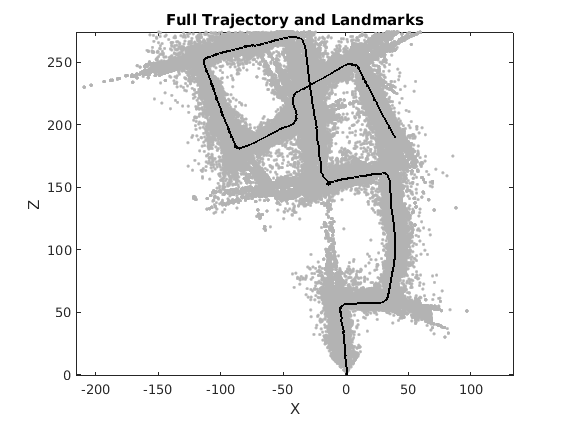
\includegraphics[width=0.6\textwidth]{Results_KITTI.png}
\caption{KITTI dataset full trajectory and landmarks}
\end{figure}

KITTI dataset shows significant scale drift without the bundle adjustment implementation. After bundle adjustment, the VO pipeline is robust enough to run to the end of the dataset. 
\section{Malaga} \label{sec:malaga}
MALAGA dataset shows scale drift even after bundle adjustment. This is thought to be from the large variations of landmark distance from the camera.

\begin{figure}[h]
\centering
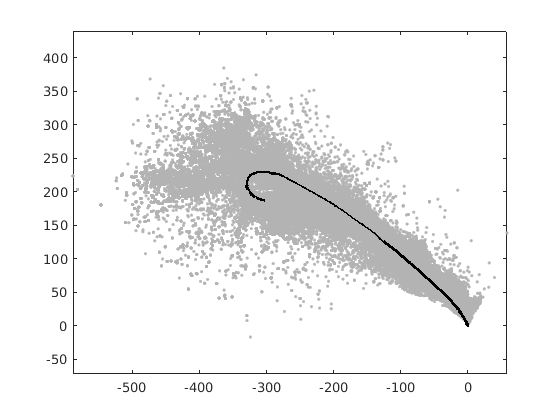
\includegraphics[width=0.6\textwidth]{Results_MALAGA.png}
\caption{MALAGA dataset full trajectory and landmarks}
\label{fig:	results_malaga}
\end{figure}

\section{Parking} \label{sec:parking}
Parking dataset shows robust performance even though the camera is facing the right angle to the direction of travel. Parking has an acculative error as the dataset has no loop even though running bundle adjustment. 

\begin{figure}[h]
\centering
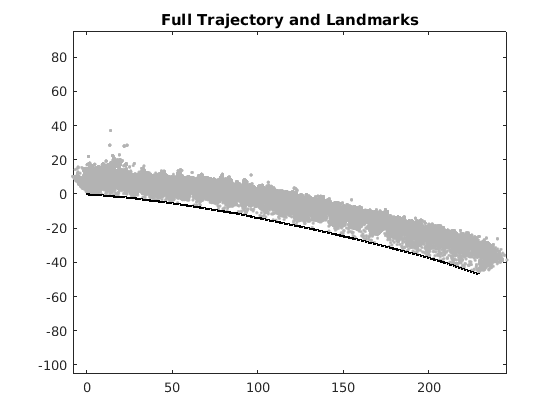
\includegraphics[width=0.6\textwidth]{Results_Parking.png}
\caption{Parking dataset full trajectory and landmarks}
\label{fig:	results_parking}
\end{figure}

\section{Custom Dataset (Seoul)} \label{sec:Custom our_dataset}

A custom dataset was constructed to verify that the visual odometry pipeline is robust enough to work in various environments. The custom dataset is based on 360 sequence of images taken from an iPhone 6s. While taking the images the camera had a fixed focal length and the images were down sampled by a factor of 0.2 for computational issues in calibrating the camera and rectifying images. Images were filmed in a narrow alley in Seoul, Republic of Korea in December 27th 2016.\newline
The successful trajectory estimation of the VO pipeline in a narrow alley with large variations of landmark distance and illumination changes shows robust performance of the VO pipeline.

\begin{figure}[h]
\centering
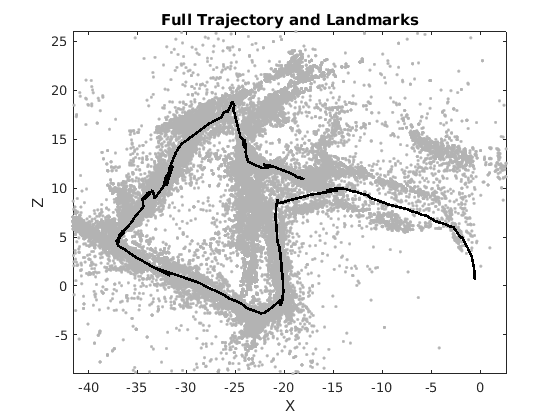
\includegraphics[width=0.6\textwidth]{Results_OWN.png}
\caption{Seoul dataset full trajectory and landmarks}
\end{figure}

\begin{figure}[h]
\centering
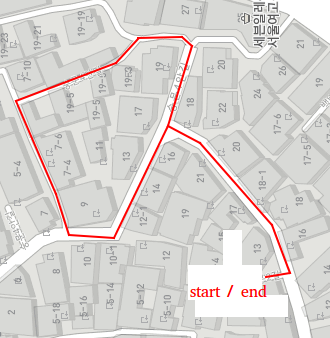
\includegraphics[width=0.5\textwidth]{seoul_ground.png}
\caption{Estimated Ground truth of Seoul dataset from Daum Map}
\end{figure}

\section*{Video Links}

\begin{itemize}
\item Youtube Playlist \url{https://www.youtube.com/playlist?list=PL4osb-habf7AwyqOOP_enbcIkzncwvSIB}
\item KITTI: \url{https://youtu.be/dS4KoISoAcE?list=PL4osb-habf7AwyqOOP_enbcIkzncwvSIB}
\item Malaga: \url{https://youtu.be/3fxA7I47CuM?list=PL4osb-habf7AwyqOOP_enbcIkzncwvSIB} 
\item Parking: \url{https://youtu.be/WfOTkpfoyzY?list=PL4osb-habf7AwyqOOP_enbcIkzncwvSIB}
\item Seoul (our data set): \url{https://youtu.be/Y0lDwR3oK0w?list=PL4osb-habf7AwyqOOP_enbcIkzncwvSIB}
\end{itemize}

\section{Conclusions}
We successfully implemented a fully working and robust monocular visual odometry pipeline as well as the additional features as the following. 

\begin{itemize}
\item An appealing visualization was implemented including keypoint tracking information, camera heading and trajectory in each frame. A full landmark and trajectory visualization is also implemented.
\item Many ideas for improving the performance of the VO pipeline. 
\item refined estimated pose by minimizing reprojection error.
\item VO pipeline verification on a custom recorded dataset.
\item Full bundle adjustment(motion and structure)
\item Not fully working but implemented loop closure module using place recognition. 
\end{itemize}